\chapter{Photoinjection}
\label{chap:photoinjection}

\section{Pump and Probe Pulse Parameters}

Understanding the transport dynamics of photoinjected carriers requires first establishing the excitation regime induced by the pump pulse. In this work, carrier generation is simulated within real-time time-dependent density functional theory (RT-TDDFT) using the SALMON code \cite{Noda_2019}. The calculations employ the PZ-LDA exchange-correlation functional \cite{Perdew1981PZ}, which, as is well known, underestimates semiconductor band gaps \cite{Onida2002ElectronicExcitations}. For crystalline silicon, according to the linear response analysis, SALMON shows a direct band gap of 2.52 eV., smaller than the real direct gap near 3.4 eV.

\begin{figure}[h!]
    \centering
    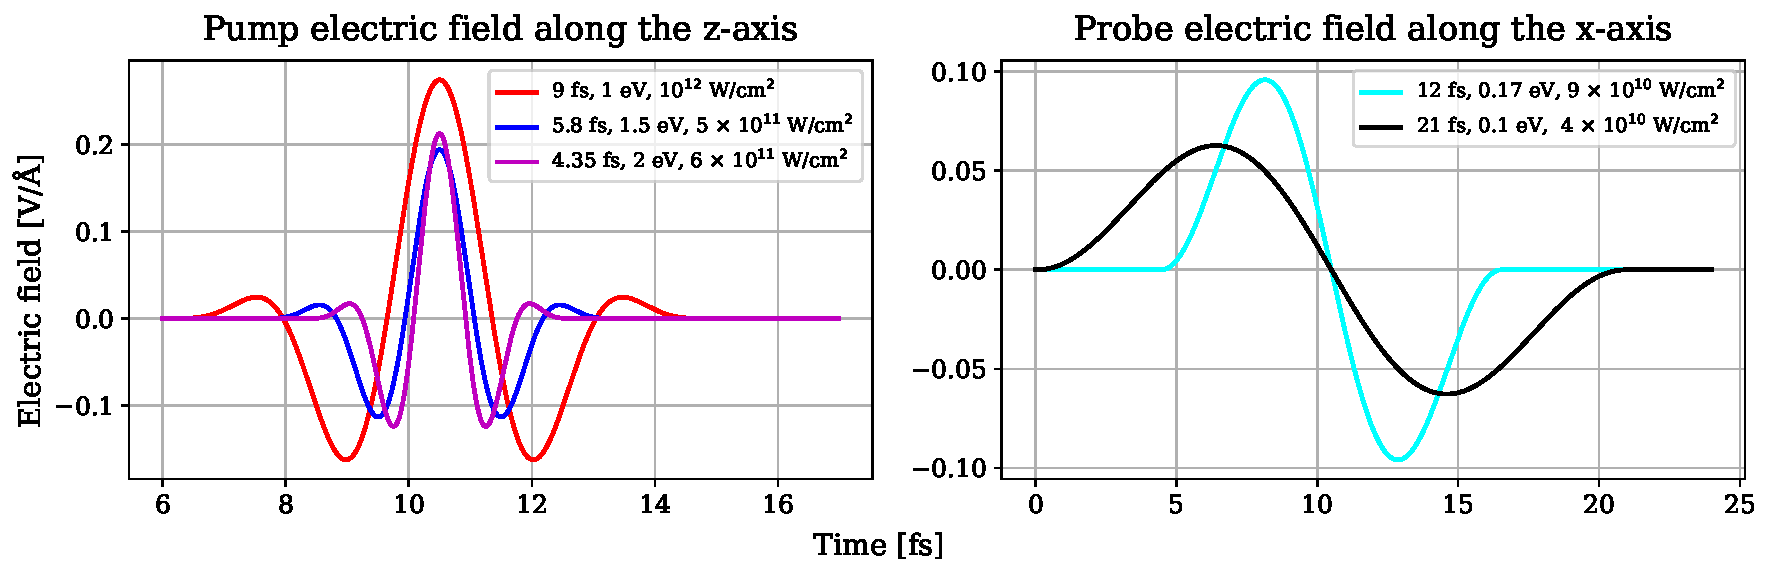
\includegraphics[width=0.9\linewidth]{all_pdf/hhg/pulses_electric_fields.pdf}
    \caption{Temporal profiles of the pump (z-polarized) and probe (x-polarized) electric fields used in the simulations. The legend indicates pulse duration, carrier frequency, and peak intensity.}
    \label{fig:pulse_fields}
\end{figure}

In this work, the pulses are introduced in the velocity gauge via the vector potential
\begin{equation}
A(t) = -\frac{E_0}{\omega}\,
\cos^n\!\left(\frac{\pi}{T}\left(t-\frac{T}{2}\right)\right)
\sin\!\left(\omega\left(t-\frac{T}{2}\right)+\varphi_{\mathrm{CEP}}\right),
\qquad (0 < t < T),
\end{equation}
where $\varphi_{\mathrm{CEP}}$ is the carrier–envelope phase, $T$ the pulse duration, $\omega$ the carrier frequency, and $E_0$ the electric-field amplitude. For the pump (probe) pulse we used $n=4 \,(2)$ and $\varphi_{\mathrm{CEP}}=0 \,(\frac{\pi}{2})$.

The corresponding electric field is obtained as
\begin{equation}
E(t) = -\frac{dA(t)}{dt}.
\label{eq:A_deriv}
\end{equation}

Figure~\ref{fig:pulse_fields} shows the electric fields of the pump and probe pulses. The pump pulse operates at carrier frequencies of 1 eV, 1.5 eV, and 2 eV. Because the TDDFT band gap is approximately 2.5 eV, excitation at 1 eV occurs in the multiphoton regime, at 1.5 eV in a reduced-order multiphoton regime, and at 2 eV close to a single-photon excitation threshold.

The nonlinear excitation mechanism in solids under strong fields has been extensively analyzed in the context of semiconductor Bloch equations and strong-field theory \cite{Golde2008HHGsolids, Vampa2015Semiclassical, Ghimire2019HHGreview}. As the photon energy approaches the band gap, the effective order of the multiphoton process decreases and the excitation dynamics progressively approach linear absorption.

Disorder accelerates this transition to single-photon excitation. The reduction of the effective band gap and the breakdown of crystal momentum conservation allow additional transitions that are forbidden in a perfect lattice. Such relaxation of $k$-selection rules in disordered semiconductors is well established in optical absorption theory \cite{MottDavis1979, Sheng2006Localization}.

It is important to emphasize that phonons are not included in the present RT-TDDFT simulations. Optical phonons in silicon have frequencies around 15 THz (period $\sim 65$ fs), while acoustic phonons correspond to even longer time scales. Since we focus on dynamics within the first 30 fs after excitation, lattice motion can be neglected. On these ultrashort time scales, carrier dynamics are governed by purely electronic processes in a static potential.

The probe pulse is chosen such that it injects a negligible number of carriers. Even if weak photoinjection occurs, its contribution is removed by subtracting the probe-only response in pump–probe simulations.

\begin{figure}[h!]
    \centering
    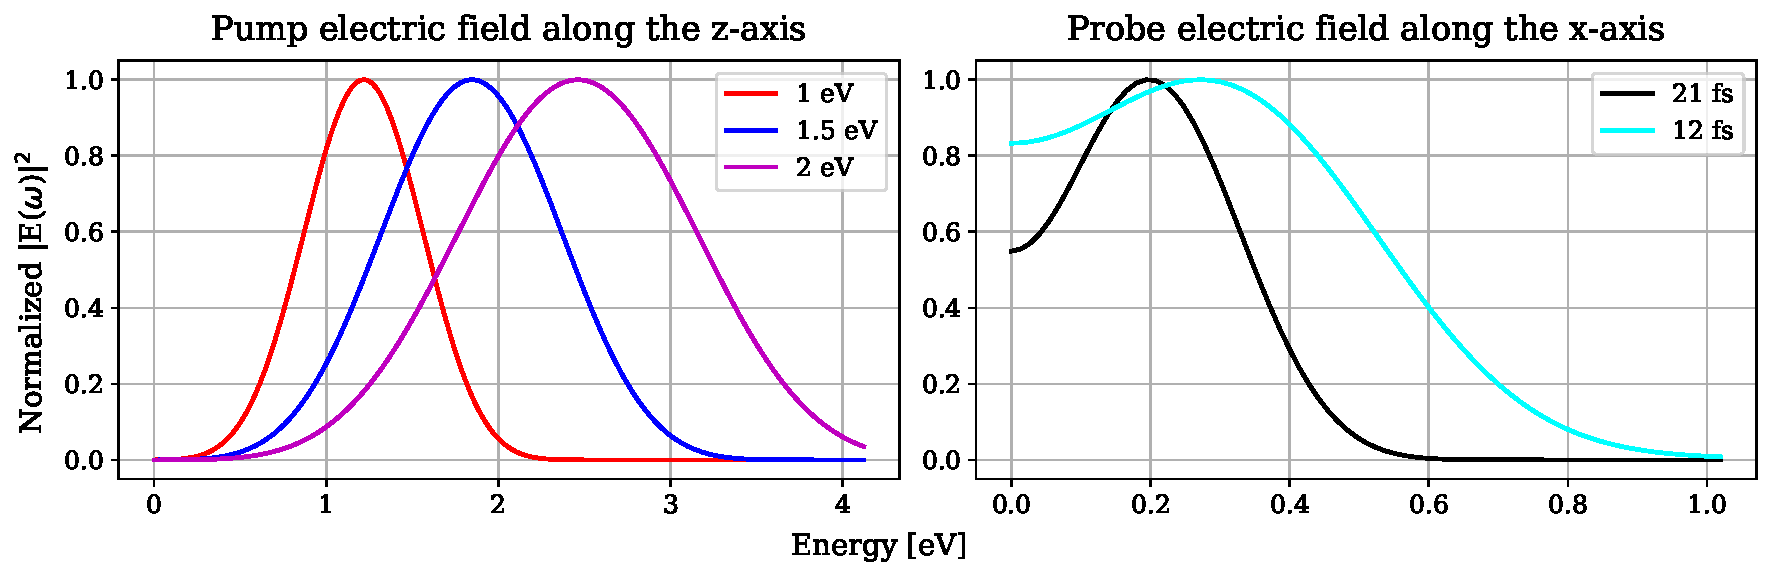
\includegraphics[width=0.9\linewidth]{all_pdf/hhg/pulses_power_spectrum_1.213_1.847_2.468_0.193_0.276.pdf}
    \caption{Power spectra of the pump and probe pulses.}
    \label{fig:pulse_spectra}
\end{figure}

Figure~\ref{fig:pulse_spectra} shows the spectral intensities $|E(\omega)|^2$ of the pulses. Because the pulses are few-cycle in duration, their spectra are broadened according to the time–frequency uncertainty relation. Such broadening is characteristic of ultrashort strong-field excitation \cite{Krausz2009Attophysics}. The spectral maxima exceed the nominal carrier frequencies due to the derivative in \eqref{eq:A_deriv}.

\section{Pump Energy}

We now analyze the electronic energy absorbed from the pump pulse and its dependence on disorder and carrier frequency.

\begin{figure}[h!]
    \centering
    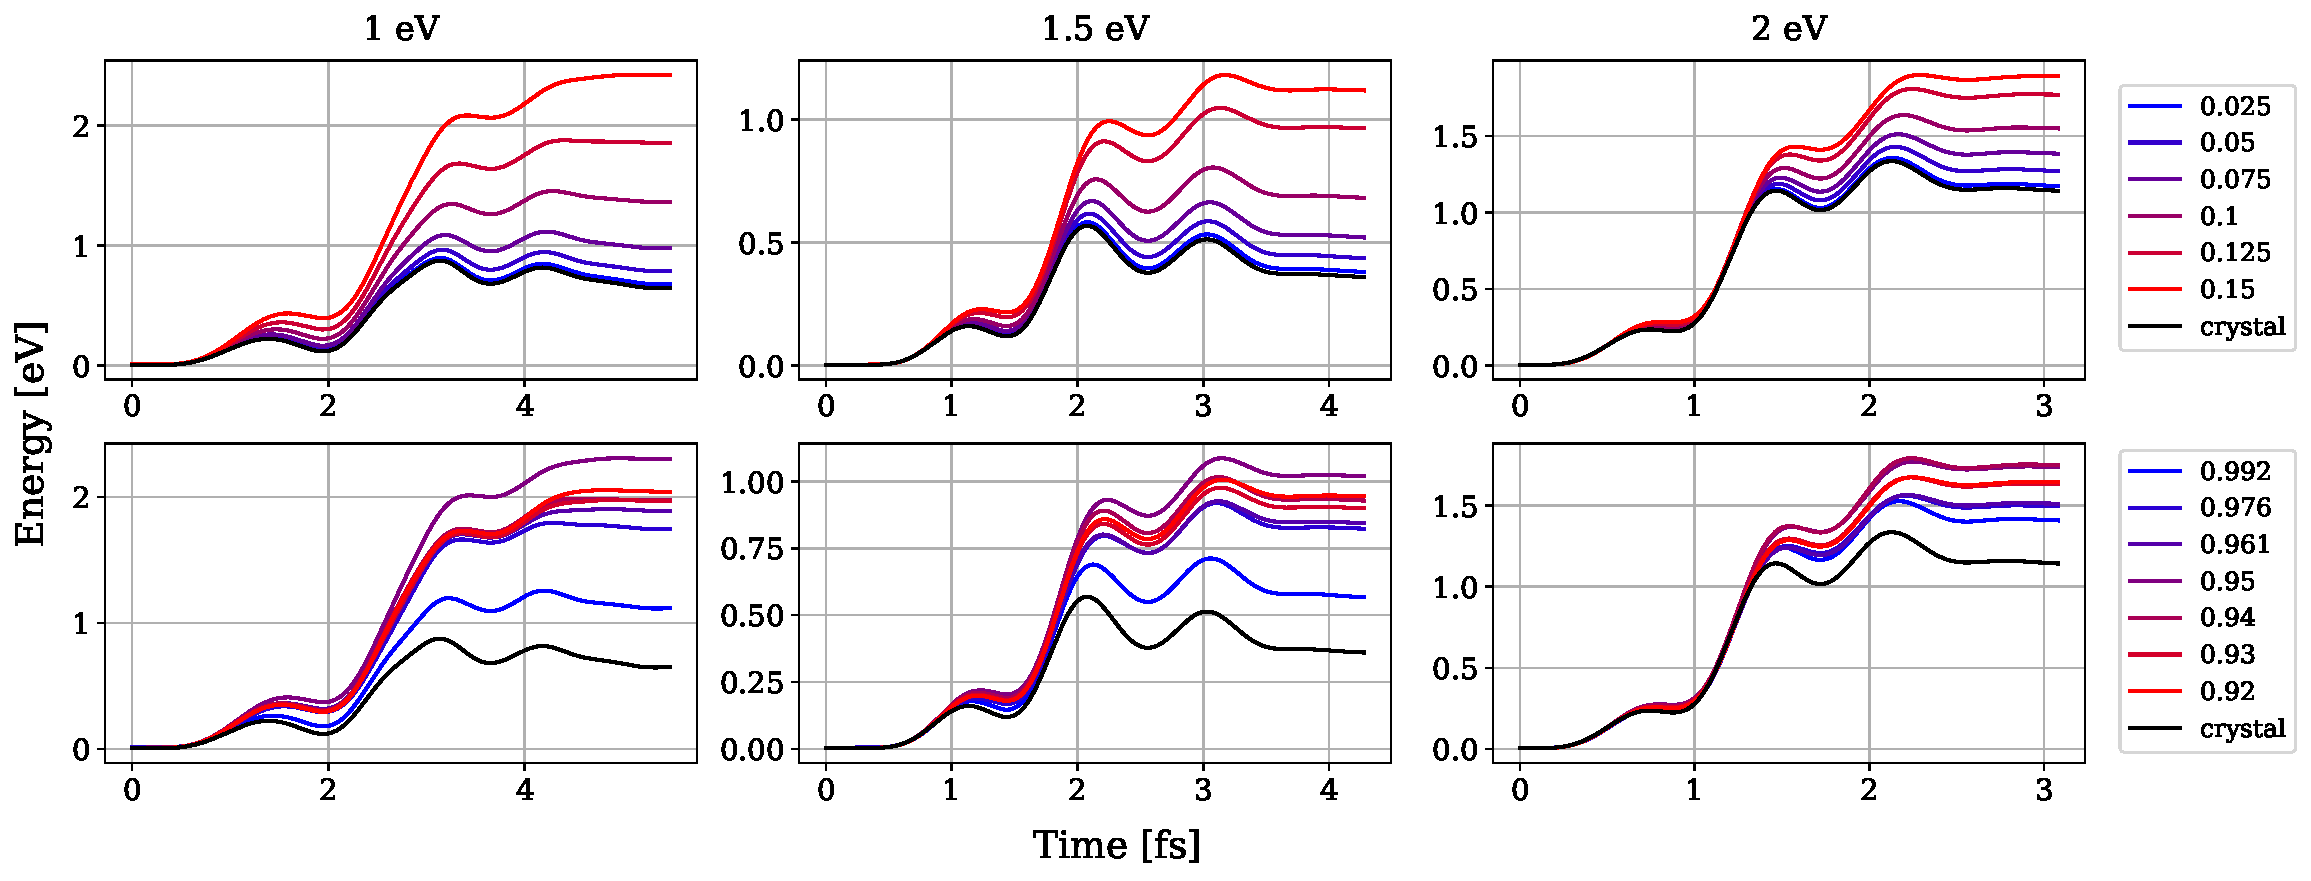
\includegraphics[width=1\linewidth]{all_pdf/energy/z/pdf/pump_energy_comparison_pump_pulse.pdf}
    \caption{Time-dependent energy absorbed from the pump pulse for different photon energies and disorder strengths. The column caption in eV indicates the carrier frequency of the pump pulse. The top row represents displacement disorder, whereas the bottom row represents amorphous disorder.}
    \label{fig:pump_energy_time}
\end{figure}

Figure~\ref{fig:pump_energy_time} shows that absorbed energy increases systematically with disorder. This increase reflects both band-gap narrowing and the relaxation of momentum conservation. Similar disorder-enhanced absorption has been reported in amorphous semiconductors and strongly perturbed crystals \cite{MottDavis1979, Sheng2006Localization}.

As the pump photon energy increases from 1 eV to 2 eV, the curvature of the energy–time curve decreases, indicating a transition toward a more linear excitation regime. This behavior is consistent with strong-field solid-state theory, where higher photon energies reduce the effective nonlinearity of the excitation channel \cite{Vampa2015Semiclassical}.

For amorphous disorder, the energy increase occurs stepwise rather than continuously. This behavior correlates with abrupt shifts in the density of states and band edges characteristic of amorphous silicon \cite{MottDavis1979}.

\begin{figure}[h!]
    \centering
    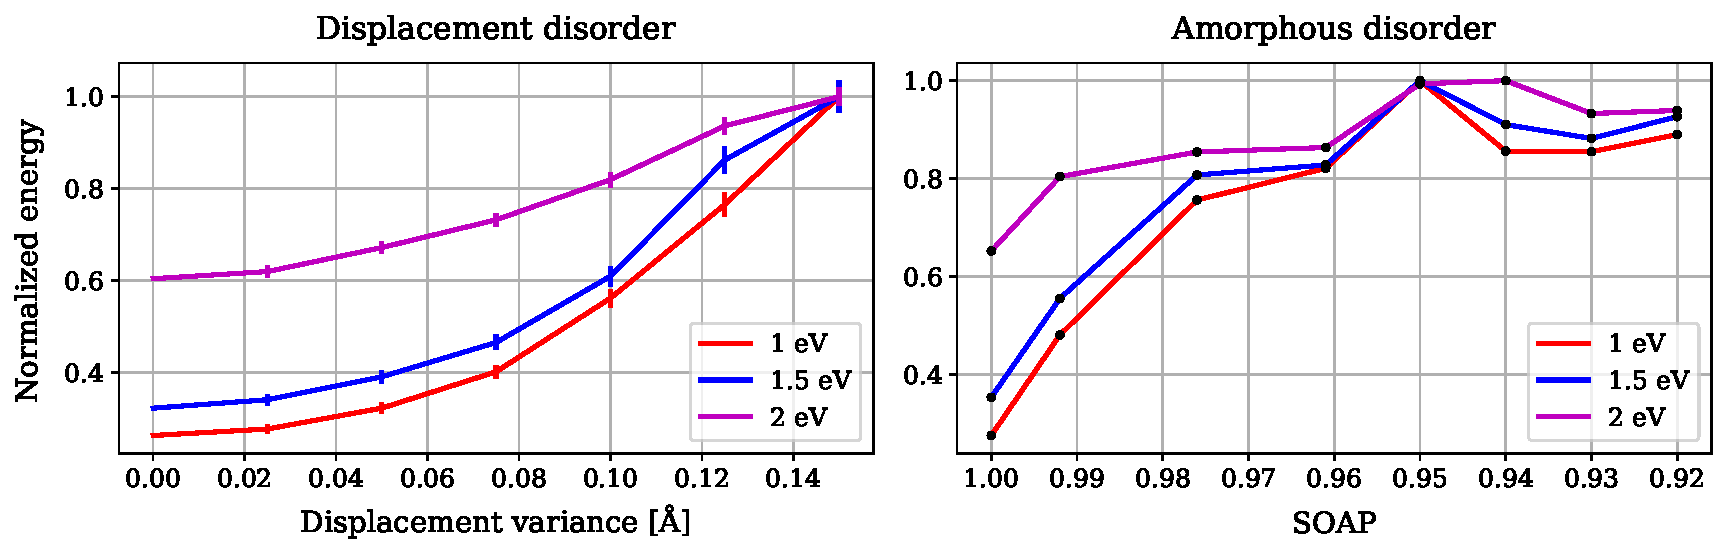
\includegraphics[width=0.9\linewidth]{all_pdf/energy/z/pdf/pump_pulse_photoinjection_energy_final_vals.pdf}
    \caption{Final absorbed pump energy values normalized to the maximum value as a function of disorder strength.}
    \label{fig:pump_energy_final}
\end{figure}

Figure~\ref{fig:pump_energy_final} shows that the spread of absorbed energies decreases with increasing photon energy. In the single-photon regime (2 eV), disorder produces smaller relative variations in excitation efficiency.

\begin{figure}[h!]
    \centering
    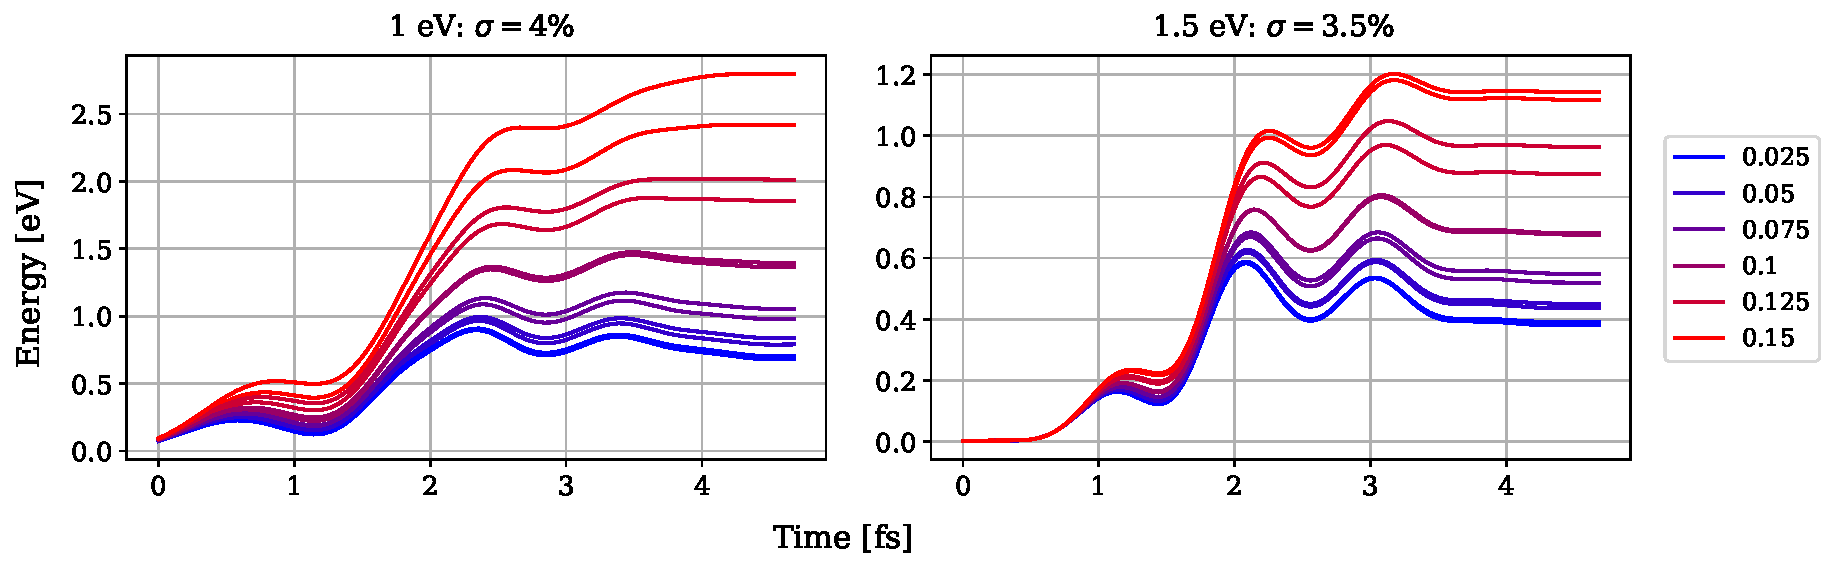
\includegraphics[width=0.9\linewidth]{all_pdf/energy/z/pdf/pump_energy_variation.pdf}
    \caption{Statistical variation of absorbed pump energy across different displacement disorder realizations.}
    \label{fig:pump_energy_variation}
\end{figure}

Figure~\ref{fig:pump_energy_variation} quantifies statistical spread across independent supercells. The variance increases with disorder but decreases with photon energy, reflecting reduced sensitivity in the single-photon regime, $\sigma$ denotes the overall relative variance of the spread of values.

\section{Pump-Induced Current}

We now examine the current induced along the pump polarization direction.

\begin{figure}[h!]
    \centering
    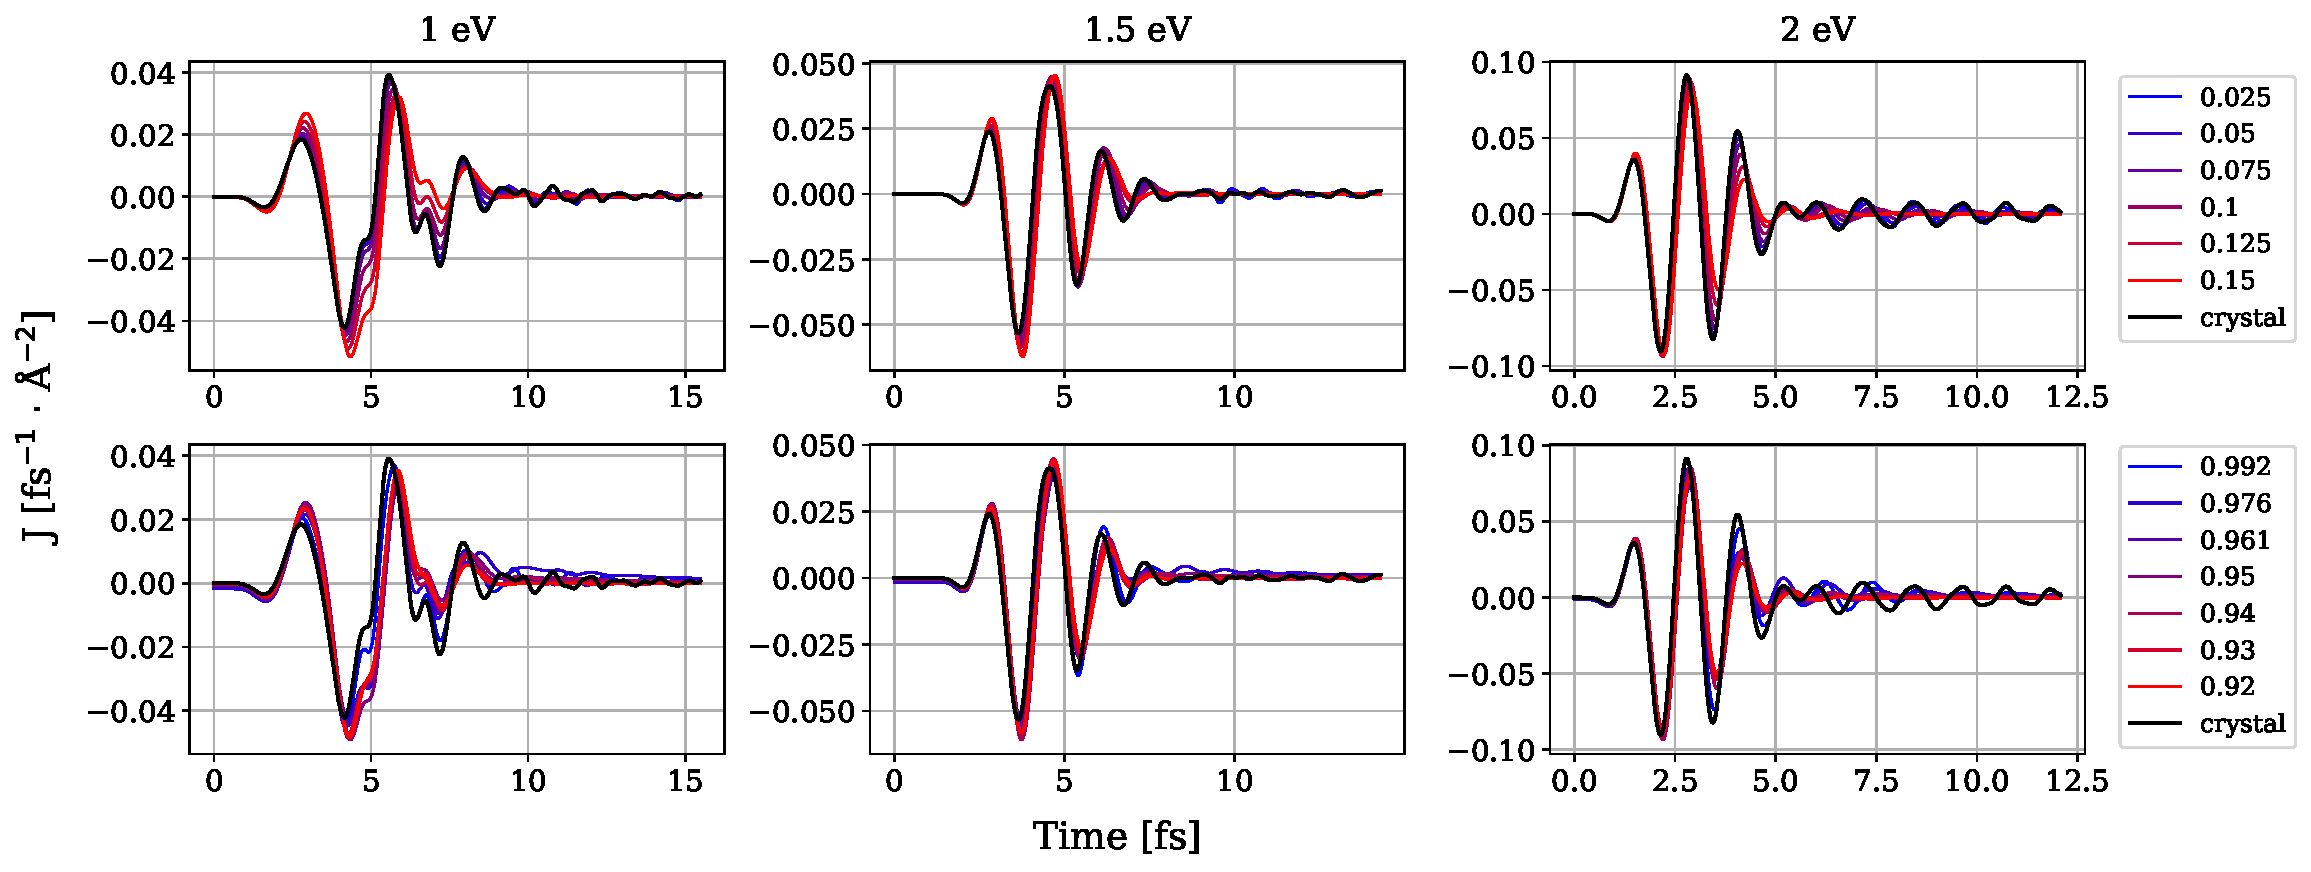
\includegraphics[width=1\linewidth]{all_pdf/current/z/pdf/pump_pulse_response_comparison.pdf}
    \caption{Time-domain current response induced by the pump pulse for increasing disorder. The column caption in eV indicates the carrier frequency of the pump pulse. The top row represents displacement disorder, whereas the bottom row represents amorphous disorder.}
    \label{fig:pump_current_time}
\end{figure}

Figure~\ref{fig:pump_current_time} shows increasing phase lag and suppression of coherent oscillations with disorder. After the pulse, oscillations decay more rapidly for stronger disorder, consistent with homogeneous dephasing due to elastic scattering.

\begin{figure}[h!]
    \centering
    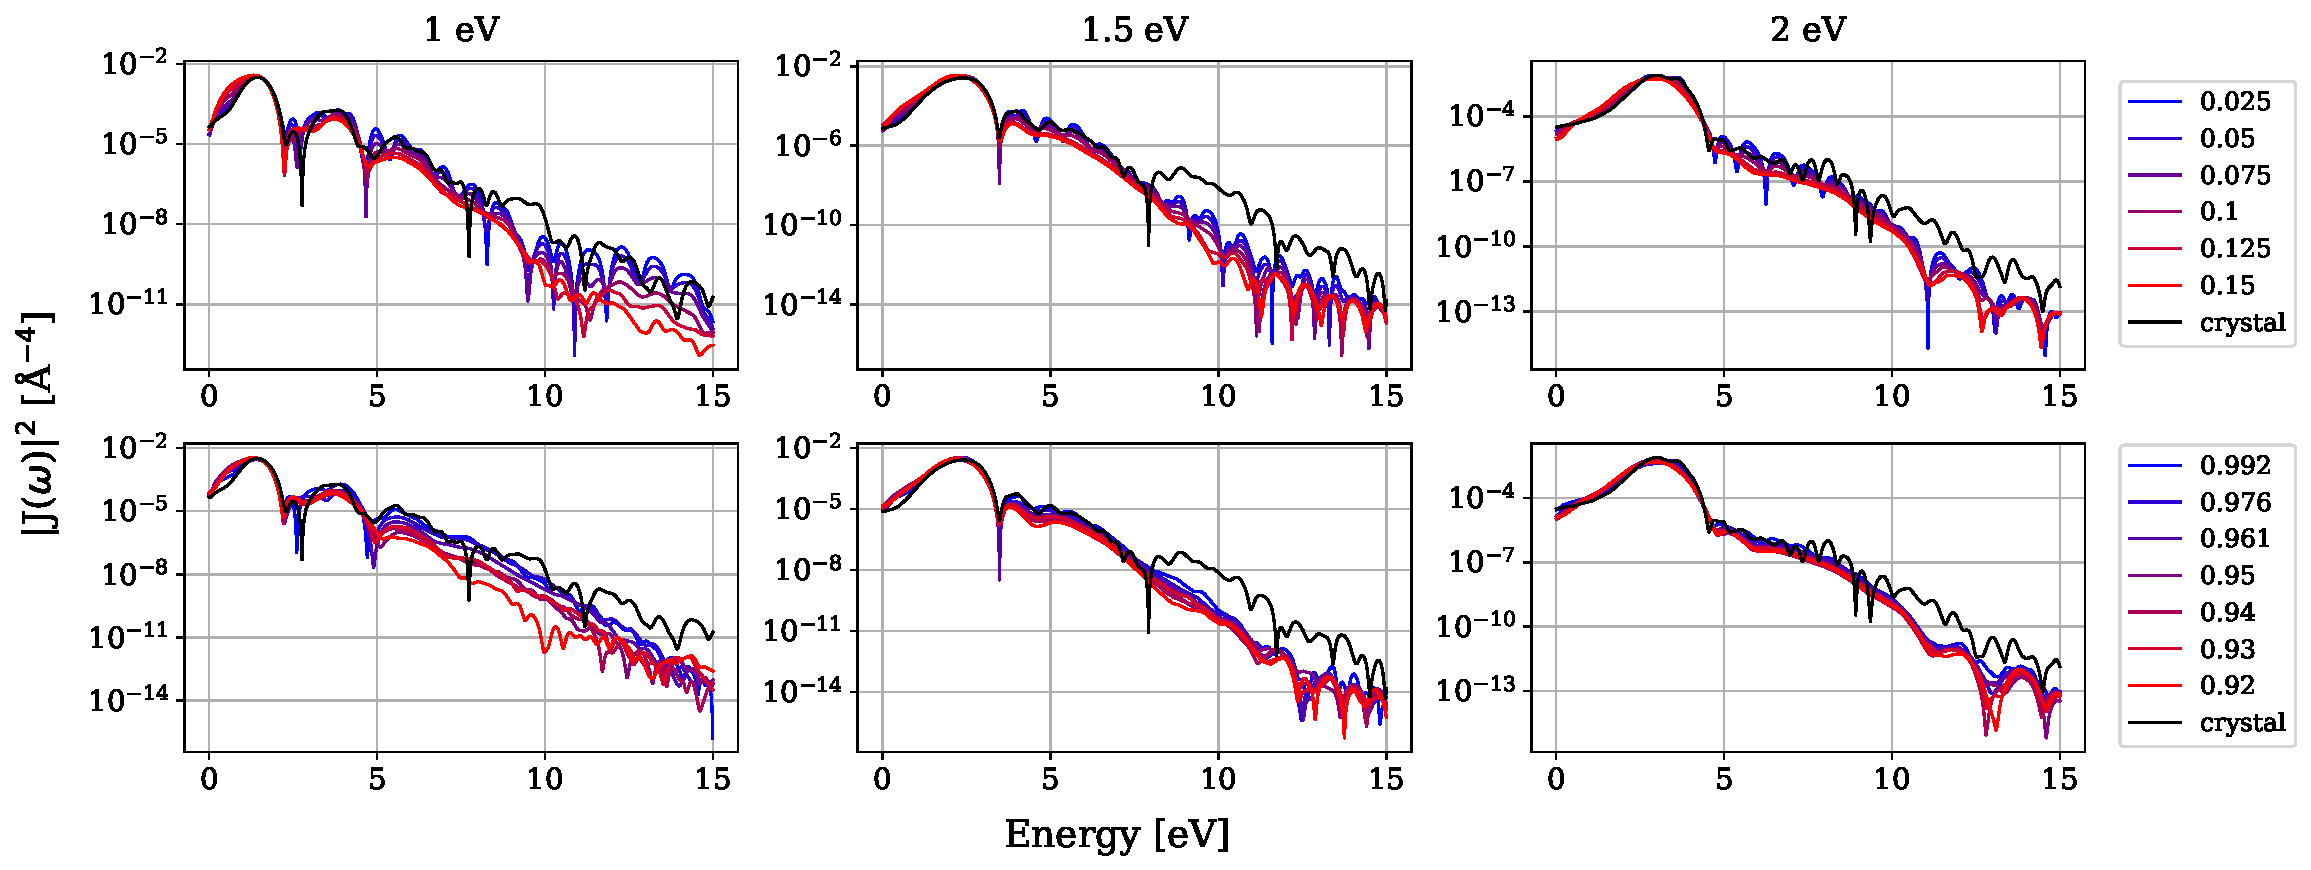
\includegraphics[width=1\linewidth]{all_pdf/hhg/z/pdf/hhg_pump_pulse_response_comparison_log.pdf}
    \caption{Logarithmic high-harmonic spectrum of the pump-induced current for different disorder strengths. The column caption in eV indicates the carrier frequency of the pump pulse. The top row represents displacement disorder, whereas the bottom row represents amorphous disorder.}
    \label{fig:pump_hhg_log}
\end{figure}

The logarithmic spectrum in Figure~\ref{fig:pump_hhg_log} demonstrates suppression of high harmonics with increasing disorder. Disorder-induced reduction of high-harmonic generation efficiency has been observed in theoretical and experimental studies of HHG in solids \cite{Vampa2015Semiclassical, Ghimire2019HHGreview}.

\begin{figure}[h!]
    \centering
    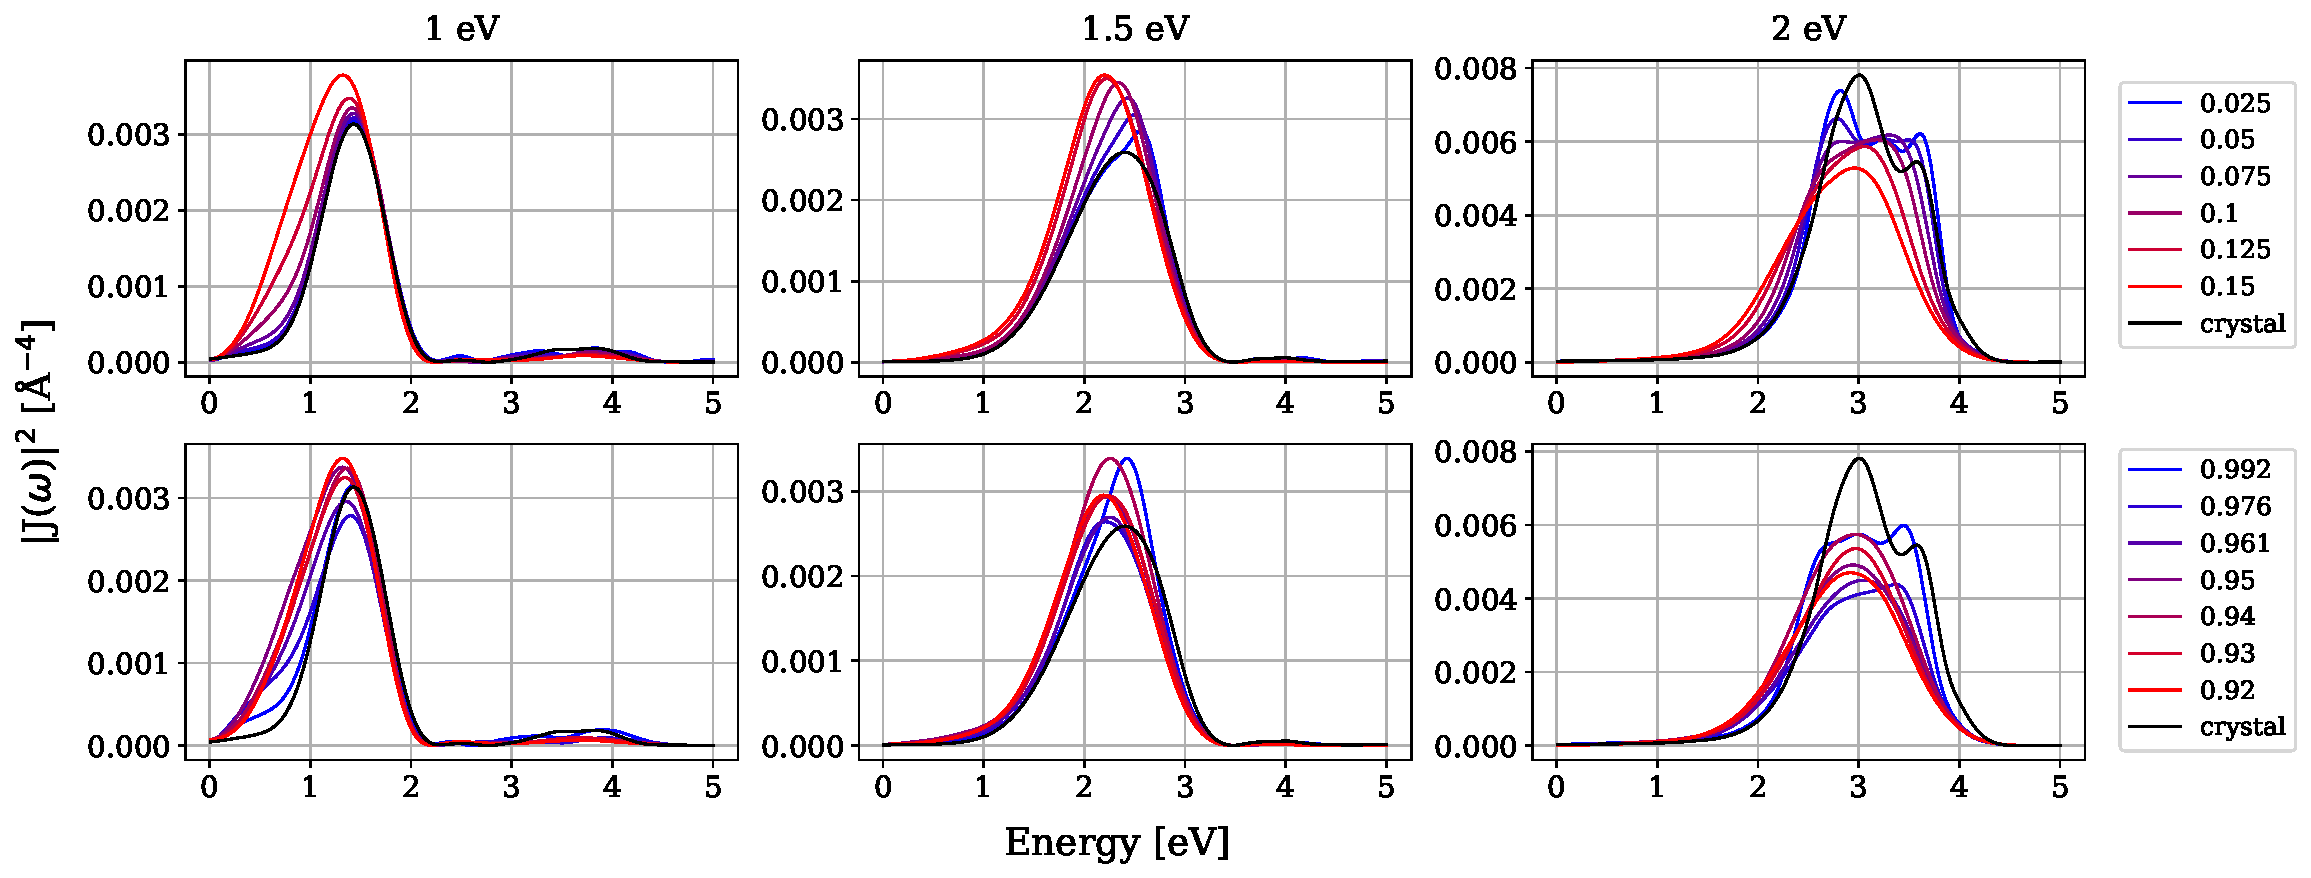
\includegraphics[width=1\linewidth]{all_pdf/hhg/z/pdf/hhg_pump_pulse_response_comparison.pdf}
    \caption{Linear-scale spectrum of the pump-induced current showing red shift and spectral broadening with disorder. The column caption in eV indicates the carrier frequency of the pump pulse. The top row represents displacement disorder, whereas the bottom row represents amorphous disorder.}
    \label{fig:pump_hhg_linear}
\end{figure}

Figure~\ref{fig:pump_hhg_linear} shows a clear red shift of the dominant spectral peak with increasing disorder, reflecting band-gap reduction. Spectral broadening accompanies the shift and can be attributed to relaxation of momentum conservation and activation of non-vertical transitions, a hallmark of disordered semiconductors \cite{MottDavis1979, Sheng2006Localization}.


\begin{figure}[h!]
    \centering
    
\includegraphics[width=0.8\linewidth]{all_pdf/lr/pdf/phi.pdf}
    \caption{
Spectral phase $\phi(\omega)$ extracted from the complex dielectric function 
$\varepsilon(\omega)=\varepsilon_1(\omega)+i\varepsilon_2(\omega)$ 
for displacement (left) and amorphous (right) disorder. 
In the energy range below $\sim 4$ eV a clear increase of the phase with increasing disorder is observed, 
reflecting disorder-induced modification of the complex optical response.
}
    \label{fig:phase_epsilon}
\end{figure}

The spectral phase shown in Fig.~\ref{fig:phase_epsilon} is obtained from the complex dielectric function
\begin{equation}
\varepsilon(\omega)=\varepsilon_1(\omega)+i\varepsilon_2(\omega),
\end{equation}
via
\begin{equation}
\phi(\omega)=\arg \sigma(\omega)
=\arctan\!\left(
\frac{-\big[\varepsilon_1(\omega)-1\big]}
{\varepsilon_2(\omega)}
\right).
\end{equation}

As visible in Fig.~\ref{fig:phase_epsilon}, in the energy range below $\sim 4$ eV
the phase increases systematically with disorder strength for both displacement
and amorphous configurations. This behavior reflects an enhanced phase lag
of the optical response associated with the growing imaginary component
of the dielectric function.

For a complete dynamical interpretation, however, it is not sufficient to
consider $\phi(\omega)$ alone. One must also analyze the first and second
spectral derivatives,
\[
\frac{d\phi}{d\omega}, \qquad 
\frac{d^2\phi}{d\omega^2},
\]
which determine the group delay and spectral dispersion, as well as the
overall spectral weight distribution. Disorder-induced spectral broadening
modifies the effective frequency content of the signal and therefore
contributes to temporal reshaping beyond a simple uniform phase shift.




\section{The Influence of the Probe Pulse on the Pump}

\begin{figure}[h!]
    \centering
    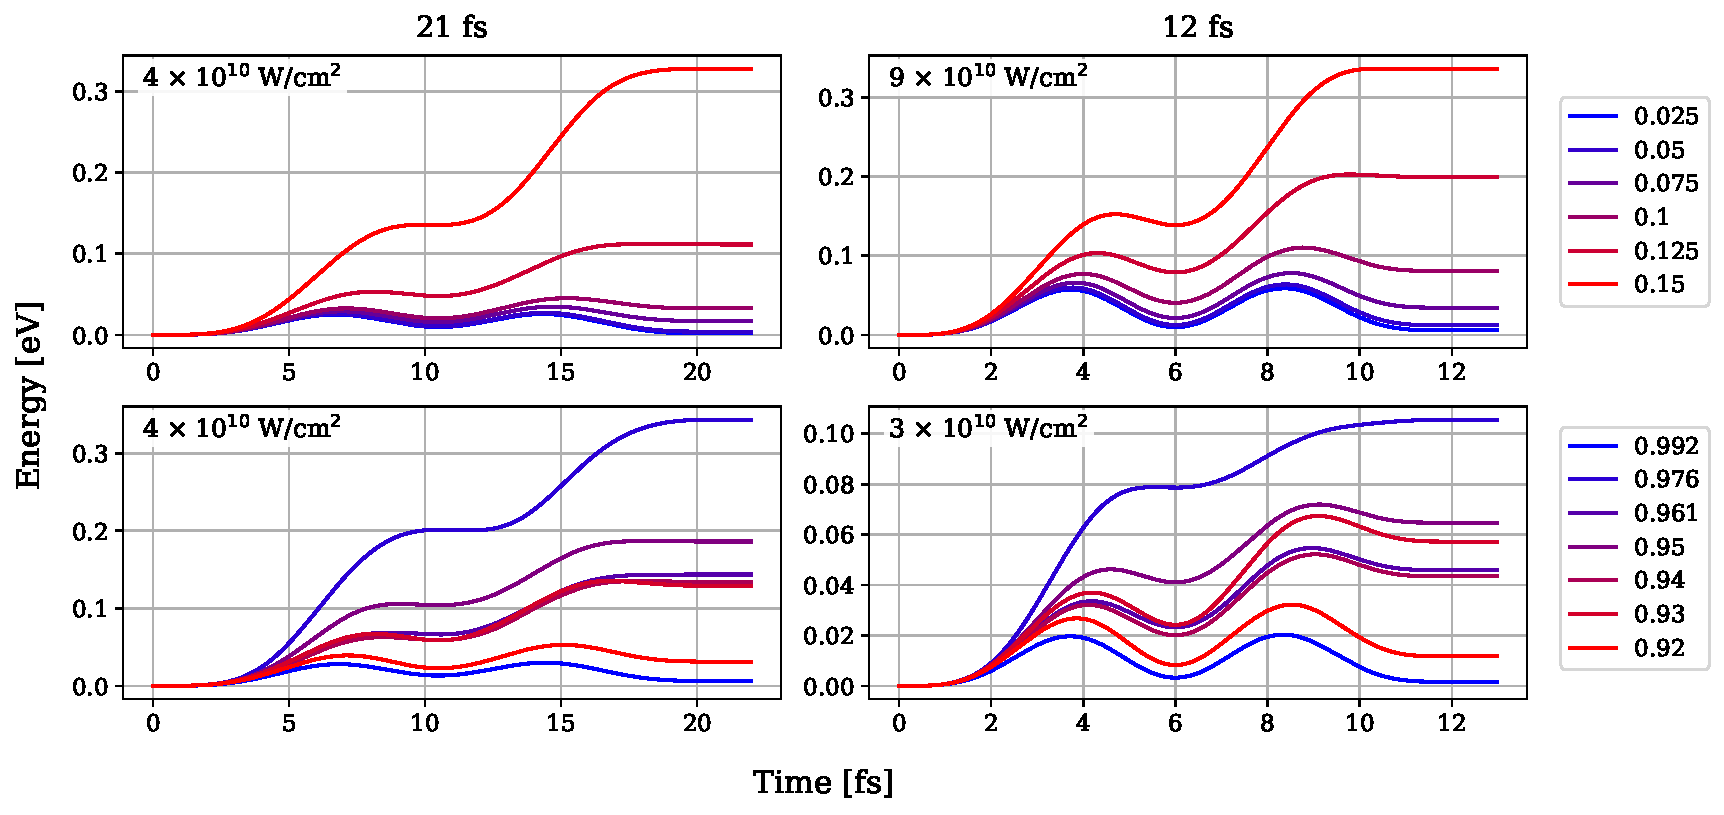
\includegraphics[width=1\linewidth]{all_pdf/energy/x/pdf/pump_energy_comparison_probe_pulse.pdf}
    \caption{Electronic energy induced by probe pulses of different duration and intensity for various disorder strengths. The top row represents displacement disorder, whereas the bottom row represents amorphous disorder.}
    \label{fig:probe_energy}
\end{figure}

Figure~\ref{fig:probe_energy} shows that for a 21 fs probe pulse with peak intensity $4 \times 10^{10}$ W/cm$^2$, photoinjection is negligible across most disorder strengths. For extreme disorder, where the effective gap approaches the probe photon energy, weak injection becomes possible. Such behavior is expected when disorder significantly modifies the density of states and relaxes selection rules \cite{MottDavis1979}.

In the subsequent analysis, we therefore use the 21 fs probe pulse as the standard configuration. Any residual probe-induced excitation is subtracted in pump–probe simulations, ensuring that the measured orthogonal current reflects purely transport dynamics.